\begin{frame}
\frametitle{What is Uncertainty Quantification (UQ)?}
\only<1>{\begin{quote}
    \Large All models are wrong, but some are useful.\\
    --George E.P. Box
\end{quote}
\bigskip

\hspace*{70pt} How inaccurate might the models be?\\
\hspace*{90pt}When are they useful in engineering problems?\\
\hspace*{110pt} How much confidence can we have in model's predictions?

\bigskip
\hspace*{130pt} \Large UQ provides a framework answering
\hspace*{140pt} these questions and making model useful.
}

\only<2>{
\begin{figure}
    \centering
    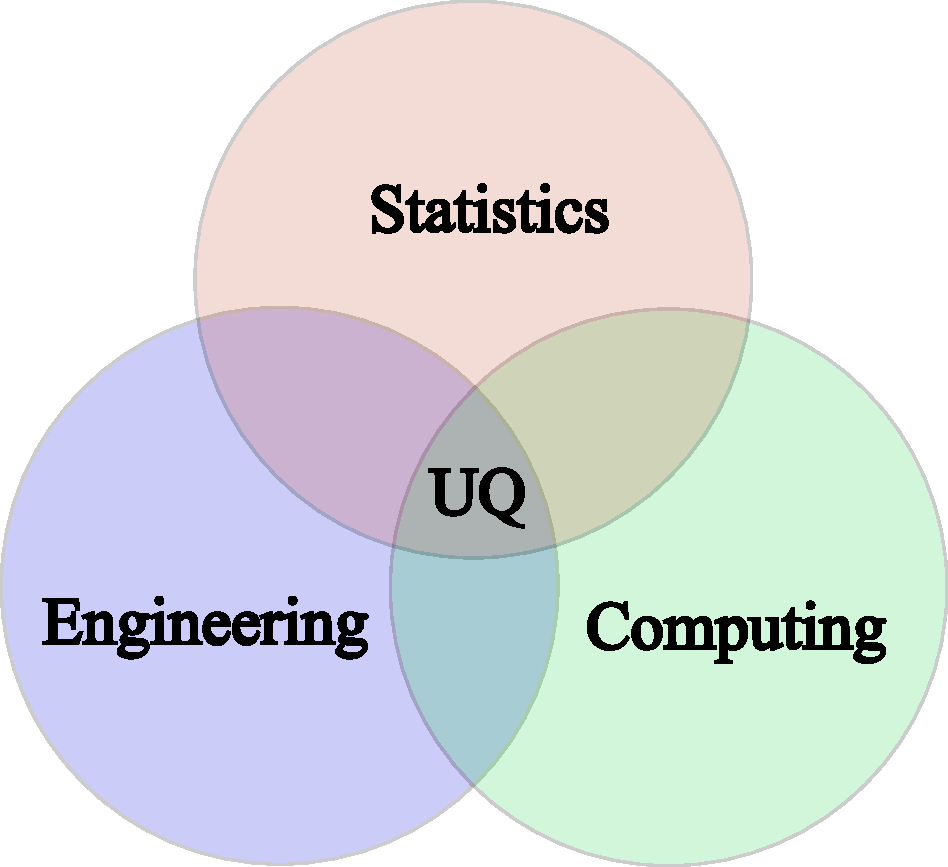
\includegraphics[width = 5.8cm]{figures/figure_UQ_subject.pdf}
    \label{fig:UQ-subject}
    \end{figure}

\begin{quote}
UQ is the science of quantitative \textcolor{red}{characterization} and \textcolor{red}{reduction} of uncertainties in both computational and real world applications\footfullcite{Saouma2021} 
\end{quote}
}



 \end{frame}